\documentclass[11pt,a4paper]{scrartcl}

% Support for UTF-8 and non-English letters require the following two
\usepackage[T1]{fontenc}
\usepackage[utf8]{inputenc}
% Font packages
\usepackage[default,defaultsans,oldstyle,proportional]{lato}
\usepackage[scaled]{beramono}
\usepackage{sfmath}
% Optimized justification via improved microtypography on character level
\usepackage{microtype}
\usepackage{ragged2e}
\usepackage[none]{hyphenat} % disable all hyphenation
\setlength{\emergencystretch}{3em} % allow extra hfill, needed if hyphenation disabled
%\overfullrule=1mm % mark overfull boxes
%\usepackage{showframe} % show edges of text areas
% Page layout
\usepackage[left=20mm,right=20mm,top=20mm,bottom=20mm,
nohead,foot=10mm]{geometry}
\usepackage{fancyvrb}
\usepackage{amsmath}

\usepackage{minted}

\usepackage{algorithm}
\usepackage{algpseudocode}
\DeclareMathOperator{\return}{\mathbf{return}}

\usepackage{tikz}
\usetikzlibrary{automata, positioning}
\tikzset{->, node distance=3cm}

\title{The PixARLang compiler}
\subtitle{CPS2000 Compiler Theory and Practice}
\author{Mark Mizzi}
\date{Last edited: \today}

\begin{document}

\maketitle

\tableofcontents

\newpage

\section{Lexing}

\subsection{Design considerations}

THere are several approaches available to the implementer when it comes to writing a hand-coded lexer.

The implementation uses a table-driven approach to lexing. This approach assumes that the micro-syntax of each token type $t_{i}$ can be specified using a regular expression $e_{i}$. The lexer emulates a particular DFSA (deterministic finite state automaton) that accepts the language specified by the following regular expression:
$$ e = e_{1} | ... | e_{k} $$

The DFSA emulated by this compiler's lexer is shown in Figure~\ref{fig:lexer-dfsa}.

\begin{figure}[H]
  \centering
  \caption{DFSA that lexes tokens in the PixAR language.}~\label{fig:lexer-dfsa}
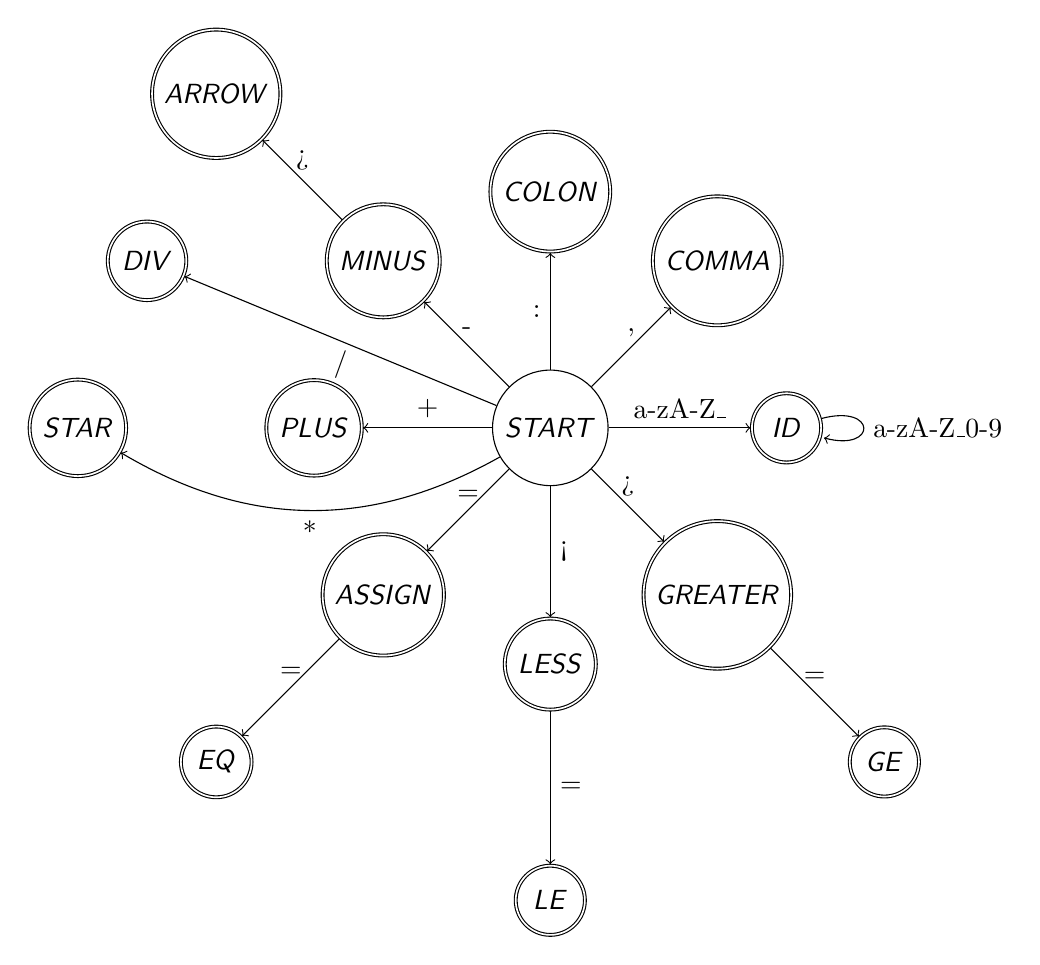
\begin{tikzpicture}
\node[state] (a) { $START$ };
\node[state, accepting, right of=a] (id) { $ID$ };
\node[state, accepting, above of=a] (colon) { $COLON$ };
\node[state, accepting, above right of=a] (comma) { $COMMA$ };
\node[state, accepting, below right of=a] (greater) { $GREATER$ };
\node[state, accepting, below of=a] (less) { $LESS$ };
\node[state, accepting, below left of=a] (assign) { $ASSIGN$ };
\node[state, accepting, left of=a] (plus) { $PLUS$ };
\node[state, accepting, above left of=a] (minus) { $MINUS$ };
\node[state, accepting, left of=minus] (div) { $DIV$ };
\node[state, accepting, left of=plus] (star) { $STAR$ };
\node[state, accepting, below right of=greater] (ge) { $GE$ };
\node[state, accepting, below of=less] (le) { $LE$ };
\node[state, accepting, below left of=assign] (eq) { $EQ$ };
\node[state, accepting, above left of=minus] (arrow) { $ARROW$ };

\draw (a) edge[above] node{a-zA-Z\_} (id)
    (id) edge[loop right] node{a-zA-Z\_0-9} (id)
    (a) edge[left] node{:} (colon)
    (a) edge[above] node{,} (comma)
    (a) edge[above] node{>} (greater)
    (greater) edge[above] node{=} (ge)
    (less) edge[right] node{=} (le)
    (a) edge[right] node{<} (less)
    (a) edge[above] node{=} (assign)
    (assign) edge[above] node{=} (eq)
    (a) edge[above] node{+} (plus)
    (a) edge[bend left, below] node{*} (star)
    (a) edge[below] node{/} (div)
    (a) edge[above] node{-} (minus)
    (minus) edge[above] node{>} (arrow);

\end{tikzpicture}
\end{figure}

The transition table of the deterministic finite state automaton is stored in an auxiliary data structure, and a ``skeleton'' function uses this table to carry out lexing itself. Pseudo-code for this function is shown in Algorithm~\ref{lst:lexer}.

\begin{algorithm}
\caption{Pseudo-code for the ``skeleton'' function at the heart of the table-driven lexer}\label{lst:lexer}
\begin{algorithmic}
  \Require $n \geq 0$
  \If{$Eof()$}
    \State $\return Token(type=END)$
  \EndIf

  \While{$!Eof()$}

  \EndWhile
\State $c \gets nextChar()$
\State $X \gets x$
\State $N \gets n$
\While{$N \neq 0$}
\If{$N$ is even}
    \State $X \gets X \times X$
    \State $N \gets \frac{N}{2}$  \Comment{This is a comment}
\ElsIf{$N$ is odd}
    \State $y \gets y \times X$
    \State $N \gets N - 1$
\EndIf
\EndWhile
\end{algorithmic}
\end{algorithm}

Several simplifying decisions were made in designing the lexer. Firstly, each valid input character was classified into a character class. The character classes are mutually exclusive, and group together characters which result in the same state transitions for each state of the DFSA. For example, the digit characters $0-9$ are classified into a single group. This greatly decreases the size of the table used. Choosing character classes is not as straightforward as it may seem, and new classes may be needed as more token types are added to the language. For example, although one may think it sufficient to create a single class for the alphabetic characters $a-zA-Z$, two classes are needed for $a-fA-F$ and $g-zG-Z$ as the former characters can appear in hexadecimal literals, whereas the latter cannot.

Secondly, a \verb!std::map! data structure was used to store the table. This allows us to encode the partial DFSA shown in Figure~\ref{fig:lexer-dfsa} directly. Transitions that would lead to an error state are ommitted from this map, and the skeleton function throws a \verb!LexerError! if it cannot make a transition while the current state is not an accepting state. The use of an array for storing the table would require transitions to an error state to be declared explicitly.

Finally, keywords are not handled directly by the table-driven portion of the lexer. Instead keywords are lexed as regular identifiers, and then filtered by another method which wraps the skeleton function. As a side effect of this design decision, the former function must also reject any identifiers which start with an underscore, which is disallowed by the language specification. This cannot be done by the skeleton function itself as certain keywords start with an underscore.

\subsection{Code organization}

\newpage

\section{Abstract Syntax tree, Visitors, and Parsing}

\subsection{Abstract syntax trees}

Abstract syntax trees are represented by an inheritance hierarchy shown in Figure~\ref{fig:ast-hierarchy}.

\begin{figure}
  \centering
  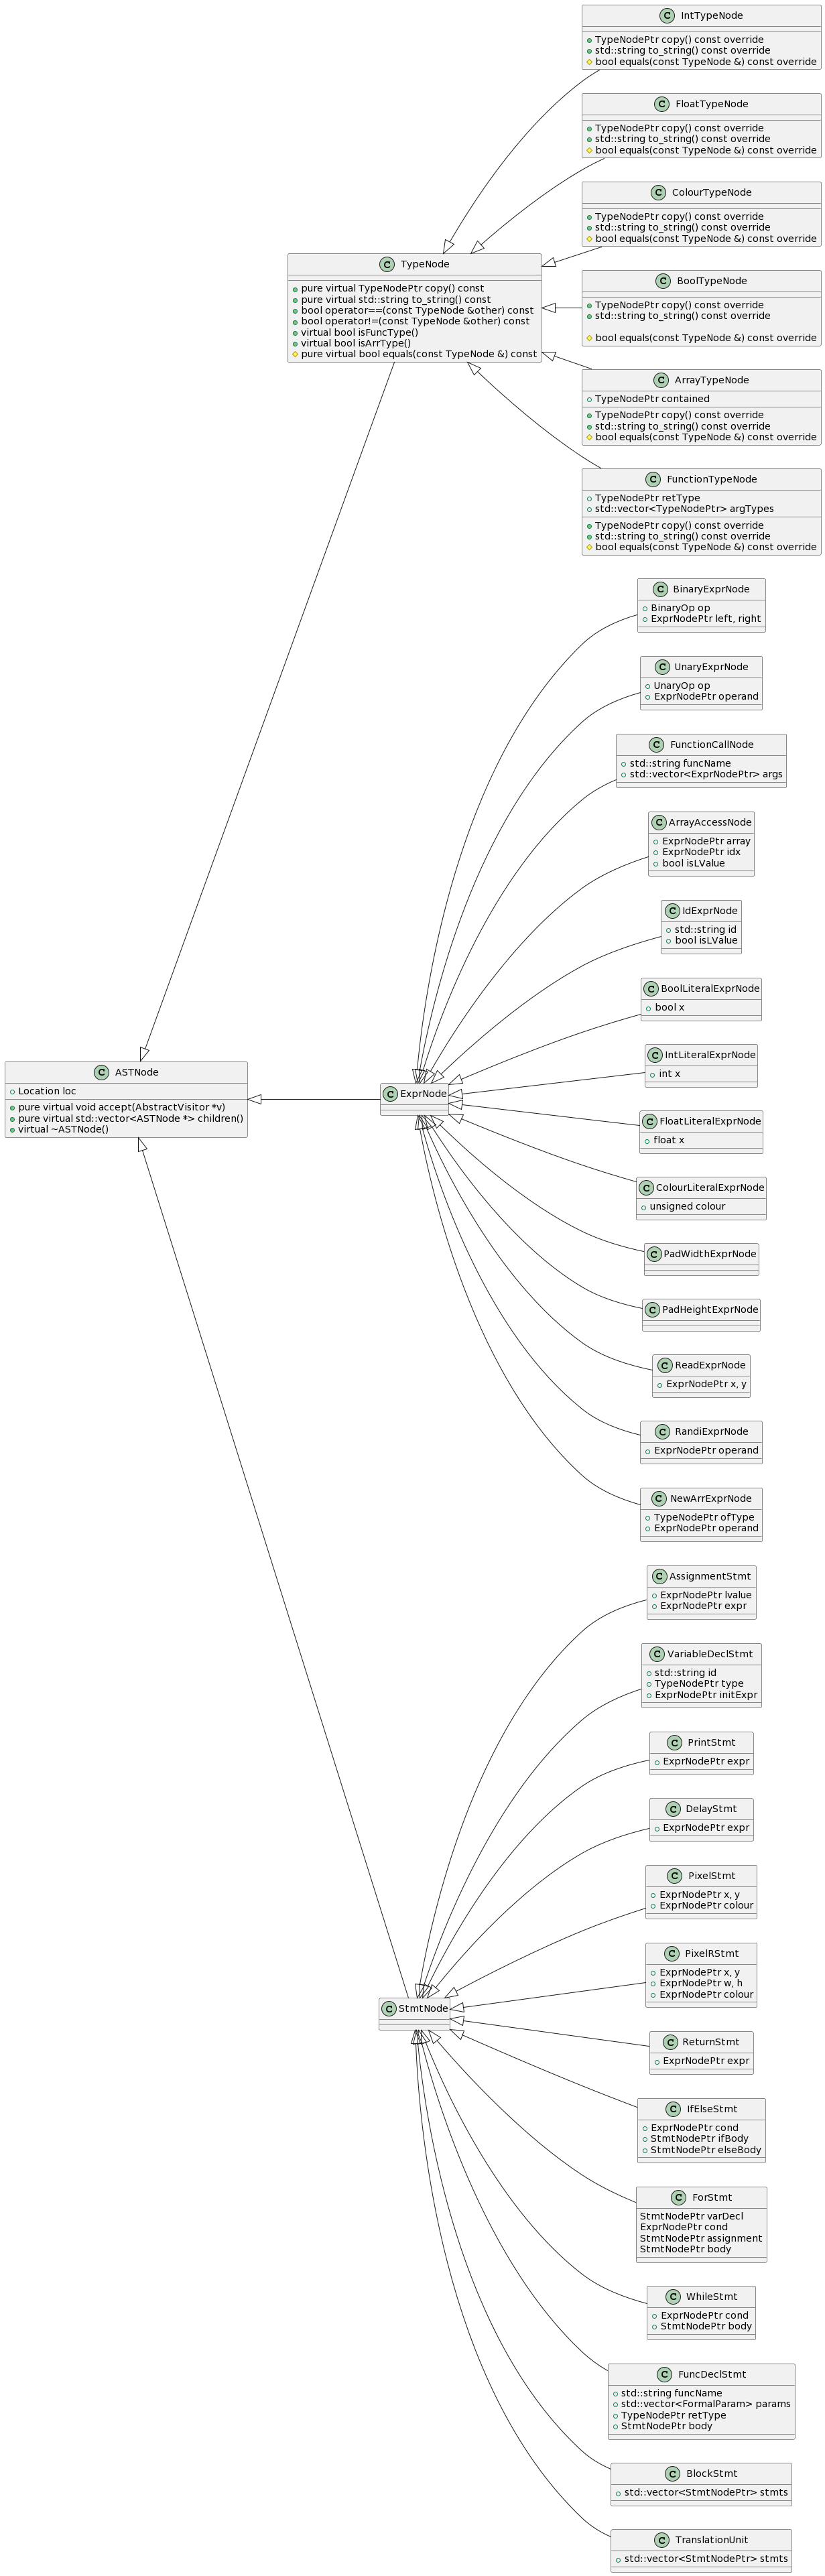
\includegraphics[height=0.95\textheight]{ast_uml}
  \caption{Inheritance hierarchy for AST nodes. Some methods are ommitted for brevity.}~\label{fig:ast-hierarchy}
\end{figure}

Every node type inherits from an \verb!ASTNode! abstract class. This class contains a \verb!Location! member that stores the position of the source code that produced the node. This allows the compiler to produce very useful error messages which indicate the location of the error to the user.

The \verb!ASTNode! type also contains a pure virtual method \verb!accept!, that subclasses must implement to support visitors. Another pure virtual method \verb!children! is implemented by subclasses to return their child nodes.

There are three direct subclasses of \verb!ASTNode!, which are themselves abstract: \verb!StmtNode!, \verb!ExprNode!, \verb!TypeNode!. These three subclasses represent the three basic kinds of syntactic structures in SIPLang: statements, expressions, and types.

Concrete subclasses of these three classes use \verb!unique_ptr! to reference child nodes.

Type nodes are used extensively in semantic checking. In order to aid this \verb!TypeNode! has additional methods \verb!copy! and \verb!to_string! which produces a deep copy of the node, and prints it in human readable form respectively.

Note that deep copying is necessary in the semantic checker due to the use of \verb!unique_ptr!. However, copying is rarely needed, and is considered a small cost compared to the convenience of using \verb!unique_ptr!.

In addition, type nodes also implement the comparision operator \verb!==!. Implementing comparision over a type hierarchy requires an unusual pattern. The implementation of \verb!operator==! in \verb!TypeNode! compares the \verb!typeid! of the two nodes being compared, and returns \verb!false! if they are not the same (dealing with the condition where the two \verb!TypeNode!s are of different types). Otherwise, a virtual \verb!equals! method is called.

In simple subclasses of \verb!TypeNode!, such as \verb!IntTypeNode! or \verb!FloatTypeNode!, this method simply returns true, as any two instances of such simple nodes are semantically equal.

For more complex subclasses, such as \verb!ArrayTypeNode!, the \verb!equals! method statically casts its argument to the type of the subclass. This is guaranteed to be type safe provided \verb!equals! is only called by \verb!operator==!. The \verb!equals! method can then perform subclass-specific equality checks, (in this case making sure the type of array elements is the same).

A subclass of \verb!TypeNode! called \verb!FunctionTypeNode! is used to represent function types during semantic checking. Nodes of this type are not produced during parsing, but are used to represent the type of function symbols.

Instances of \verb!TypeNode! also have \verb!isFuncType! and \verb!isArrType! methods which can be used to check whether a \verb!TypeNode! is an \verb!ArrayTypeNode! or a \verb!FunctionTypeNode! respectively.

\subsection{The Visitor Pattern}

The visitor pattern is widely used in compilers to cleanly separate an abstract syntax tree data structure from the implementation of algorithms that need to traverse it.

The SIPLang compiler employs a fairly pedestrian implementation of the visitor pattern. Visitors subclass an \verb!AbstractVisitor! class, which has an overloaded pure virtual \verb!visit! method for each concrete derived class of \verb!ASTNode!, which is passed as an argument (by reference):

\begin{minted}{c++}
class AbstractVisitor {
public:
  virtual void visit(IntTypeNode &node) = 0;
  // ...
  virtual void visit(TranslationUnit &node) = 0;
\end{minted}

\verb!ASTNode! contains a pure virtual method called \verb!accept!, which takes a pointer to an \verb!AbstractVisitor! instance. Each concrete derived class of \verb!ASTNode! implements \verb!accept! to call the version of the \verb!visit! method that accepts its type:

\begin{minted}{c++}
  void accept(AbstractVisitor *v) override { v->visit(*this); }
\end{minted}

In addition \verb!AbstractVisitor! has concrete methods \verb!visitChildren! and \verb!rvisitChildren!. These methods both take a pointer to an \verb!ASTNode! instance, and use its \verb!children! method to visit each of its child nodes (by calling the \verb!accept! method on each of the children). \verb!rvisitChildren! traverses the \verb!vector! of children in reverse order (this proves useful during code generation).

Concrete subclasses of \verb!AbstractVisitor! are used to generate XML for a parsed AST, for semantic checking, as well as for code generation.

\subsection{Design considerations for the parser}

The compiler uses a recursive descent parser which directly produces the AST.

Parse errors are handled by \verb!throw!ing an instance of \verb!ParserError!. This class inherits from the generic \verb!CompilationError! class, and reports an error message along with the location in the source file where the error originated.

Logic for the parser is encapsulated in a \verb!Parser! class. This class has two methods which are fundamental to parsing: \verb!peek! and \verb!consume!.

\verb!peek! takes an integer parameter \verb!i!, and looks ahead \verb!i! tokens in the token stream. Since tokens are obtained one by one from the lexer, and there is no way to look-ahead without consuming a token, the parser keeps an internal queue of tokens. If a lookahead smaller than the size of the queue is requested, \verb!peek! simply returns the appropriate token from the queue. Otherwise, the method gets the required tokens from the lexer and pushes them onto the queue, returning the last one.

Similarly \verb!consume! checks the internal queue. If it is non-empty, it pops and returns the token at the front of the queue. Otherwise, it gets the next token from the lexer, and returns it.

The parsing functions interact with the token stream through these functions. Due to the limited expressivity of SIPLang, the largest lookahead required is of 2 tokens. This lookahead of 2 tokens is used to differentiate between function calls (in which case a lookahead of 2 yields a \verb!(! token), or array accesses (in which case a lookahead of 2 yields a \verb![! token), or identity expressions.

In order to aid parsing, a \verb!CHECK_TOKEN! macro is used to check the type of a token with an expected type, and throw an appropriate \verb!ParserError! if the types don't match.

In general, duplicate or redundant checks are avoided in the parsing functions. For example, the method \verb!parseWhile! which parses a \verb!while! statement is only invoked by the \verb!parseStatement! function when the next lookahead token is a \verb!while! keyword token. The method therefore consumes a token without checking it, assuming that it is a \verb!while! keyword token.

In addition, recursion is avoided where possible. For example, where the EBNF of SIPLang specifies that zero or more repetitions of a non-terminal are part of a valid production rule, a loop is used to implement parsing of these repetitions. This makes construction of the AST simpler; nodes are simply accumulated into a vector, and then passed directly to the node constructor.

The following snippet shows the implementation of block parsing, which demonstrates the features described above:

\begin{minted}{c++}
ast::StmtNodePtr Parser::parseBlock() {
  Location loc = consume().loc; // consume {

  std::vector<ast::StmtNodePtr> stmts;

  while (peek(0).type != lexer::RBRACE_TOK) {
    stmts.push_back(std::move(parseStatement()));
  }

  Location endloc = consume().loc; // consume }.

  return std::make_unique<ast::BlockStmt>(std::move(stmts), loc.merge(endloc));
}
\end{minted}

Firstly, note that the first token is consumed without checking that it is indeed a \verb!{! token. Its location is saved to a variable, as it is needed to construct the location of the node produced.

Secondly, note that statements are parsed using a \verb!while! loop, and collected in a \verb!vector!.

Finally, the \verb!}! token is consumed, and a new \verb!BlockStmt! node is constructed using the \verb!StmtNode!s parsed. There is no check to confirm that the last token consumed is a \verb!}! token, as this is the terminating condition of the \verb!while! loop.

\newpage

\section{XML generation}

XML generation is implemented using a subclass of \verb!AbstractVisitor! called \verb!XMLVisitor!. The code is contained in \verb!xml_visitor.hh!/\verb!xml_visitor.cc!.

Generating XML is straightforward, but tedious, so two macros, \verb!XML_ELEM_WITH_CHILDREN!, and \verb!XML_ELEM_WITH_CONTENT!, are used to ease the job. One of the macros generates XML for AST nodes which have children (using, among other things, the \verb!visitChildren! method), while the other generates XML for leaves of the AST tree, where the content between XML tags is derived directly from the node.

Each of these macros writes to a \verb!std::stringstream! in the \verb!XMLVisitor! class, which is used to store the incrementally generated XML. An \verb!indent! member variable is used to keep track of the current indentation level of the XML being produced.

The generated XML includes source locations for each of the AST nodes. In addition, special characters are sanitized. For example, the \verb!<! character is converted to \verb!&gt;!. This allows external programs, such as a browser, to correctly parse the XML produced.

Once an AST has been visited, the generated XML can be extracted from the visitor using the \verb!xml! method, which simply produces a \verb!string! from the \verb!stringstream! member.

Below is the XML output from the compiler for the simple program

\begin{minted}{text}
__pixelr 0, 0, 3, 4, #ff0000;
\end{minted}

that prints a red rectangle in the bottom left corner of the PixAR VM screen:

\begin{minted}{xml}
<TranslationUnit loc="[1:0]-[1:29]">
 <PixelRStmt loc="[1:0]-[1:29]">
  <IntLiteralExprNode loc="[1:9]-[1:10]">0</IntLiteralExprNode>
  <IntLiteralExprNode loc="[1:12]-[1:13]">0</IntLiteralExprNode>
  <IntLiteralExprNode loc="[1:15]-[1:16]">3</IntLiteralExprNode>
  <IntLiteralExprNode loc="[1:18]-[1:19]">4</IntLiteralExprNode>
  <ColourLiteralExprNode loc="[1:21]-[1:28]">16711680</ColourLiteralExprNode>
 </PixelRStmt>
</TranslationUnit>
\end{minted}

\newpage

\section{Semantic checking}

\newpage

\section{Code generation and Optimizations}

\end{document}
